\documentclass{article}

\title{Laboratorio - Esercizio con SFC}
\author{Benedetta Vitale ed Emilio Meroni}
\date{12 maggio 2024}

\usepackage[italian]{babel}  % Lingua
\usepackage{tabularx} %per le tabelle
\usepackage{booktabs} %per le linee
\usepackage{graphicx} %per le immagini
\usepackage{pdfpages} %include pdf
\usepackage{amsmath} %uso simboli matematici

\begin{document}

\maketitle  % Comando per generare il titolo

\tableofcontents

\begin{figure}[b]
    \centering
    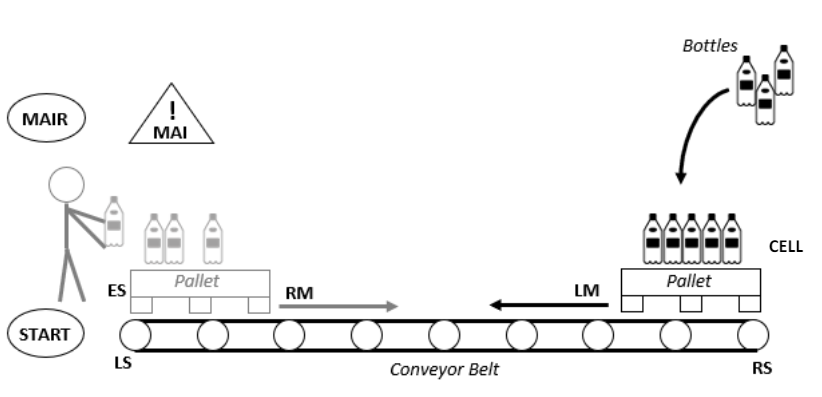
\includegraphics[width = 0.8 \linewidth]{schematico.png}
    \caption{Schema di funzionamento}
    \label{fig:schematico}
\end{figure}
\section{Itroduzione}
Il sistema per cui abbiamo fatto lo schema di controllo tramite \textit{SFC}, gestisce il carico e lo scarico delle bottiglie su dei pallet [figura: \ref{fig:schematico}].
\\

Si hanno due zone principali (carico e scarico), collegate da un nastro trasportatore. Quella a destra, serve per caricare automaticamente 10 bottiglie su un pallet, le quali vengono contate da una fotocellula. Quella a sinistra, invece, serve per lo scarico del pallet, da parte di un operatore.

Al momento che il pallet è scarico, rilevato da un sensore, e l'operatore clicca il pulsante START, il pallet torna verso la zona di carico ricominciando il ciclo di lavoro.

\section{Definizione Variabili}
In questa sezione definiamo e spieghiamo le diverse variabili che abbiamo utilizzato, in particolare le raggruppiamo per:
\begin{itemize}
    \item Input e Output
    \item Stati
    \item Valori e Costanti
\end{itemize}

\subsection{Input e Output}
Di seguito presentiamo la tabella [\ref{tab:input_output}] contenente tutti gli input e output che abbiamo utilizzato:
\begin{center}
    \begin{tabular}{l l l l }
        \toprule
        \textbf{Nome} & \textbf{Tipologia} & \textbf{Descrizione}                           \\
        \midrule
        \midrule
        RM            & Output             & Motore nastro trasportatore verso destra       \\
        \midrule
        LM            & Output             & Motore nastro trasportatore verso sinistra     \\
        \midrule
        MAI           & Output             & Allarme che indica la manutenzione             \\
        \midrule
        CELL          & Input              & Fotocellula che rileva il passaggio delle      \\
                      &                    & bottiglie                                      \\
        \midrule

        RS            & Input              & Sensore di fine corsa destro                   \\
        \midrule
        LS            & Input              & Sensore di fine corsa sinistro                 \\
        \midrule
        ES            & Input              & Sensore che rileva se il pallet è vuoto (ES=1) \\
        \midrule
        start         & Input              & Pulsante per avviare il nastro trasportatore   \\
                      &                    & verso destra                                   \\
        \midrule
        MAIR          & Input              & Pulsante per il reset della manutenzione       \\
        \bottomrule
    \end{tabular}
    \label{tab:input_output}
\end{center}

\subsection{Stati del Sistema}
\begin{center}
    \begin{tabular}{l l l l }
        \toprule
        \textbf{Nome}   & \textbf{Descrizione}                                   \\
        \midrule
        \midrule
        inizio          & Stato iniziale, il quale viene eseguito solo all'avvio \\
                        & della macchina                                         \\
        \midrule
        attesaBottiglia & Stato nel quale siamo in attesa del passaggio di una   \\
                        & bottiglia                                              \\
        \midrule
        conta           & Incremento di 1 il contatore delle bottiglie         \\
        \midrule
        attesaSicurezza & Stato che garantisce i 5 secondi, per motivi di        \\
                        & sicurezza                                              \\
        \midrule
        vaASinistra     & Stato in cui il nastro trasportatore si muove verso    \\
                        & sinistra                                               \\
        \midrule
        scarico         & Momento in cui l'operatore sta scaricando il pallet    \\
        \midrule
        vaADestra       & Stato in cui il nastro trasportatore si muove verso    \\
                        & destra                                                 \\
        \midrule
        manutenzione    & Stato di manutenzione                                  \\
        \bottomrule
    \end{tabular}
    \label{tab:stati}
\end{center}

\subsection{Altre Variabili}
\begin{center}
    \begin{tabular}{l l c l}
        \toprule
        \textbf{Nome} & \textbf{Tipo} & \textbf{Descrizione}                               \\
        \midrule
        \midrule
        x             & USINT         & Contatore delle bottiglie per il carico del pallet \\
        \midrule
        botPerMan     & USINT         & Contatore per la manutenzione                      \\
        \bottomrule
    \end{tabular}
\end{center}


\section{Assunzioni}
Abbiamo deciso di creare uno stato iniziale, chiamato \textit{inizio}, dove si entra solo una volta, all'accesione della macchina. Serve per assicurarsi che il pallet sia a destra inizialmente, infatti la transizione viene regolata da \textit{RS}(fotocellula presenza pallet destra); in uscita dallo stato \textit{inizio} abbiamo aggiunto il reset delle variabili: \textit{x} e \textit{botPerMan}.  
\\

Dato che, nel testo non era specificato quando inserire la manutenzione, abbiamo deciso di inserirla durante il conteggio delle bottiglie; quindi il blocco del pulsante \textit{start} viene fatto in modo implicito.


\section{Problematiche}
Durante lo svolgimento abbiamo affrontato qualche problematica, in particolare:
\begin{enumerate}
    \item Nella transizione \textit{"attesaSicurezza.t $>=$ T\#5s"}, ci dava un errore, dicendo che \textit{attesaSicurezza} doveva essere dichiarata come variabile, ma è uno stato. Di conseguenza abbiamo capito che il problema era che: lo stato non aveva nessuna azione da eseguire; perciò abbiamo dovuto inserire la variabile: "\textit{nonFaNulla}", che non fa nulla.
    \item Durante il debugging abbiamo notato che se $x = 10$ e, nello stesso momento $botPerMan = 25$, il programma andava in \textit{attesaSicurezza} e non in \textit{manutenzione}; perciò abbiamo inserito nella transizione anche: "AND botPerMan$<$25" (che abbiamo anche applicato alla transizione che da \textit{conta} porta in \textit{attesaBottiglia}).
    \item Infine, abbiamo separato le 2 casistiche in cui siamo in manutenzione:
          \begin{itemize}
              \item $x < 10$: in questo caso, quando la manutenzione finisce (a seguito della pressione di \textit{MAIR}), ritorniamo ad attendere una nuova bottiglia.
              \item $x \geq 10$ (che saranno ogni n cicli, dove n è multiplo di 6):  in questo caso, essendo già dieci le bottiglie, finita la manutenzione, andremo in \textit{attesaSicurezza}.
          \end{itemize}
\end{enumerate}

\section{Programma}
Di seguito presentiamo il nostro programma \textit{SFC}
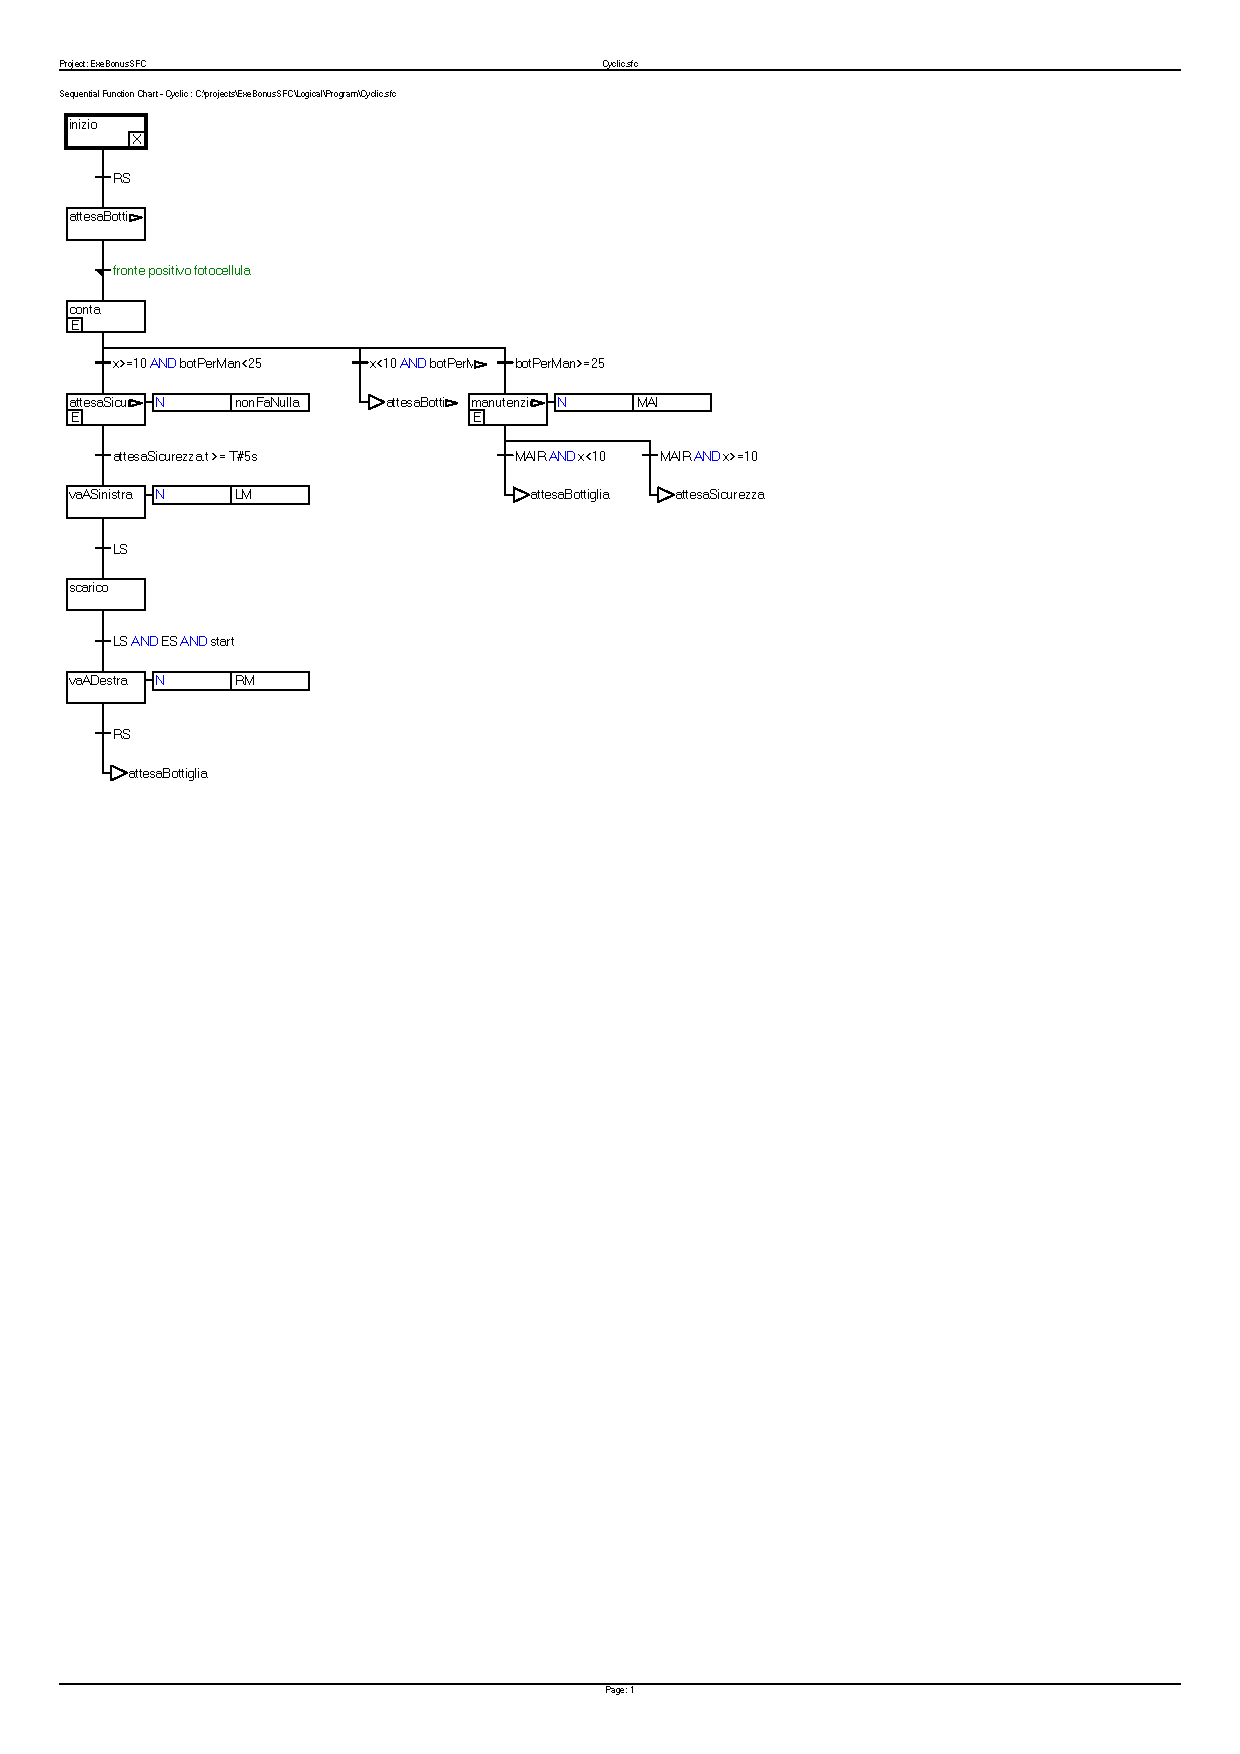
\includepdf[pages=-]{print.pdf}



\end{document}